\documentclass[journal]{IEEEtran}


% correct bad hyphenation here
\hyphenation{op-tical net-works semi-conduc-tor}
\usepackage{amsmath}
\usepackage{comment}
\usepackage{booktabs}
\usepackage{graphicx}
%\usepackage{cases}
%\usepackage{subeqnarray}

\begin{document}
%
% paper title
% Titles are generally capitalized except for words such as a, an, and, as,
% at, but, by, for, in, nor, of, on, or, the, to and up, which are usually
% not capitalized unless they are the first or last word of the title.
% Line-breaks \\ can be used within to get better formatting as desired.
% Do not put math or special symbols in the title.
\title{A Voting Based Method with Convolutional Neural Networks for No-reference Smartphone Camera Photos Quality Assessment}
%
%
% author names and IEEE memberships
% note positions of commas and non-breaking spaces ( ~ ) LaTeX will not break
% a structure at a ~ so this keeps an author's name from being broken across
% two lines.
% use \thanks{} to gain access to the first footnote area
% a separate \thanks must be used for each paragraph as LaTeX2e's \thanks
% was not built to handle multiple paragraphs
%

\author{Zhengke~Wu, Ruofeng~Liu, Jiaqi~Ma
\thanks{This work is part of the final project of CS386 Digital Image Processing in SJTU, 2020 Fall.}}

% make the title area
\maketitle

% As a general rule, do not put math, special symbols or citations
% in the abstract or keywords.
\begin{abstract}
Smartphone has been one of the most popular digital devices in the past decades and a huge number of photos are taken by smartphone cameras nowadays. As consumers are paying more and more attention to smartphone cameras, image quality assessment (IQA) has become an important but challenging task for smartphone manufacturers. In this work, we propose a voting based method with convolutional neural networks to help assess smartphone camera photos quality without reference images. First, we select small patches from high-resolution camera photos to reduce computational costs. Then we input these patches in pair into our voting model that determines which patch has a higher quality and votes for it. Finally, with all these voting results, we rank the quality of all images. Experimental results show that our method can achieve satisfying performance and outperform some previous methods on testing dataset. 
\end{abstract}

% Note that keywords are not normally used for peerreview papers.
\begin{IEEEkeywords}
No-reference Image quality assessment (NR IQA), Convolutional neural network (CNN), Smartphone camera photo
\end{IEEEkeywords}

\IEEEpeerreviewmaketitle

\section{Introduction}

As this is just a course project report, we don't think it's necessary to include a lengthy and boring introduction section. 

So that's it. Let's focus more on our proposed method and experiments.

\section{Proposed Method}

\subsection{Problem Formulation}
\begin{figure*}
    \centering
    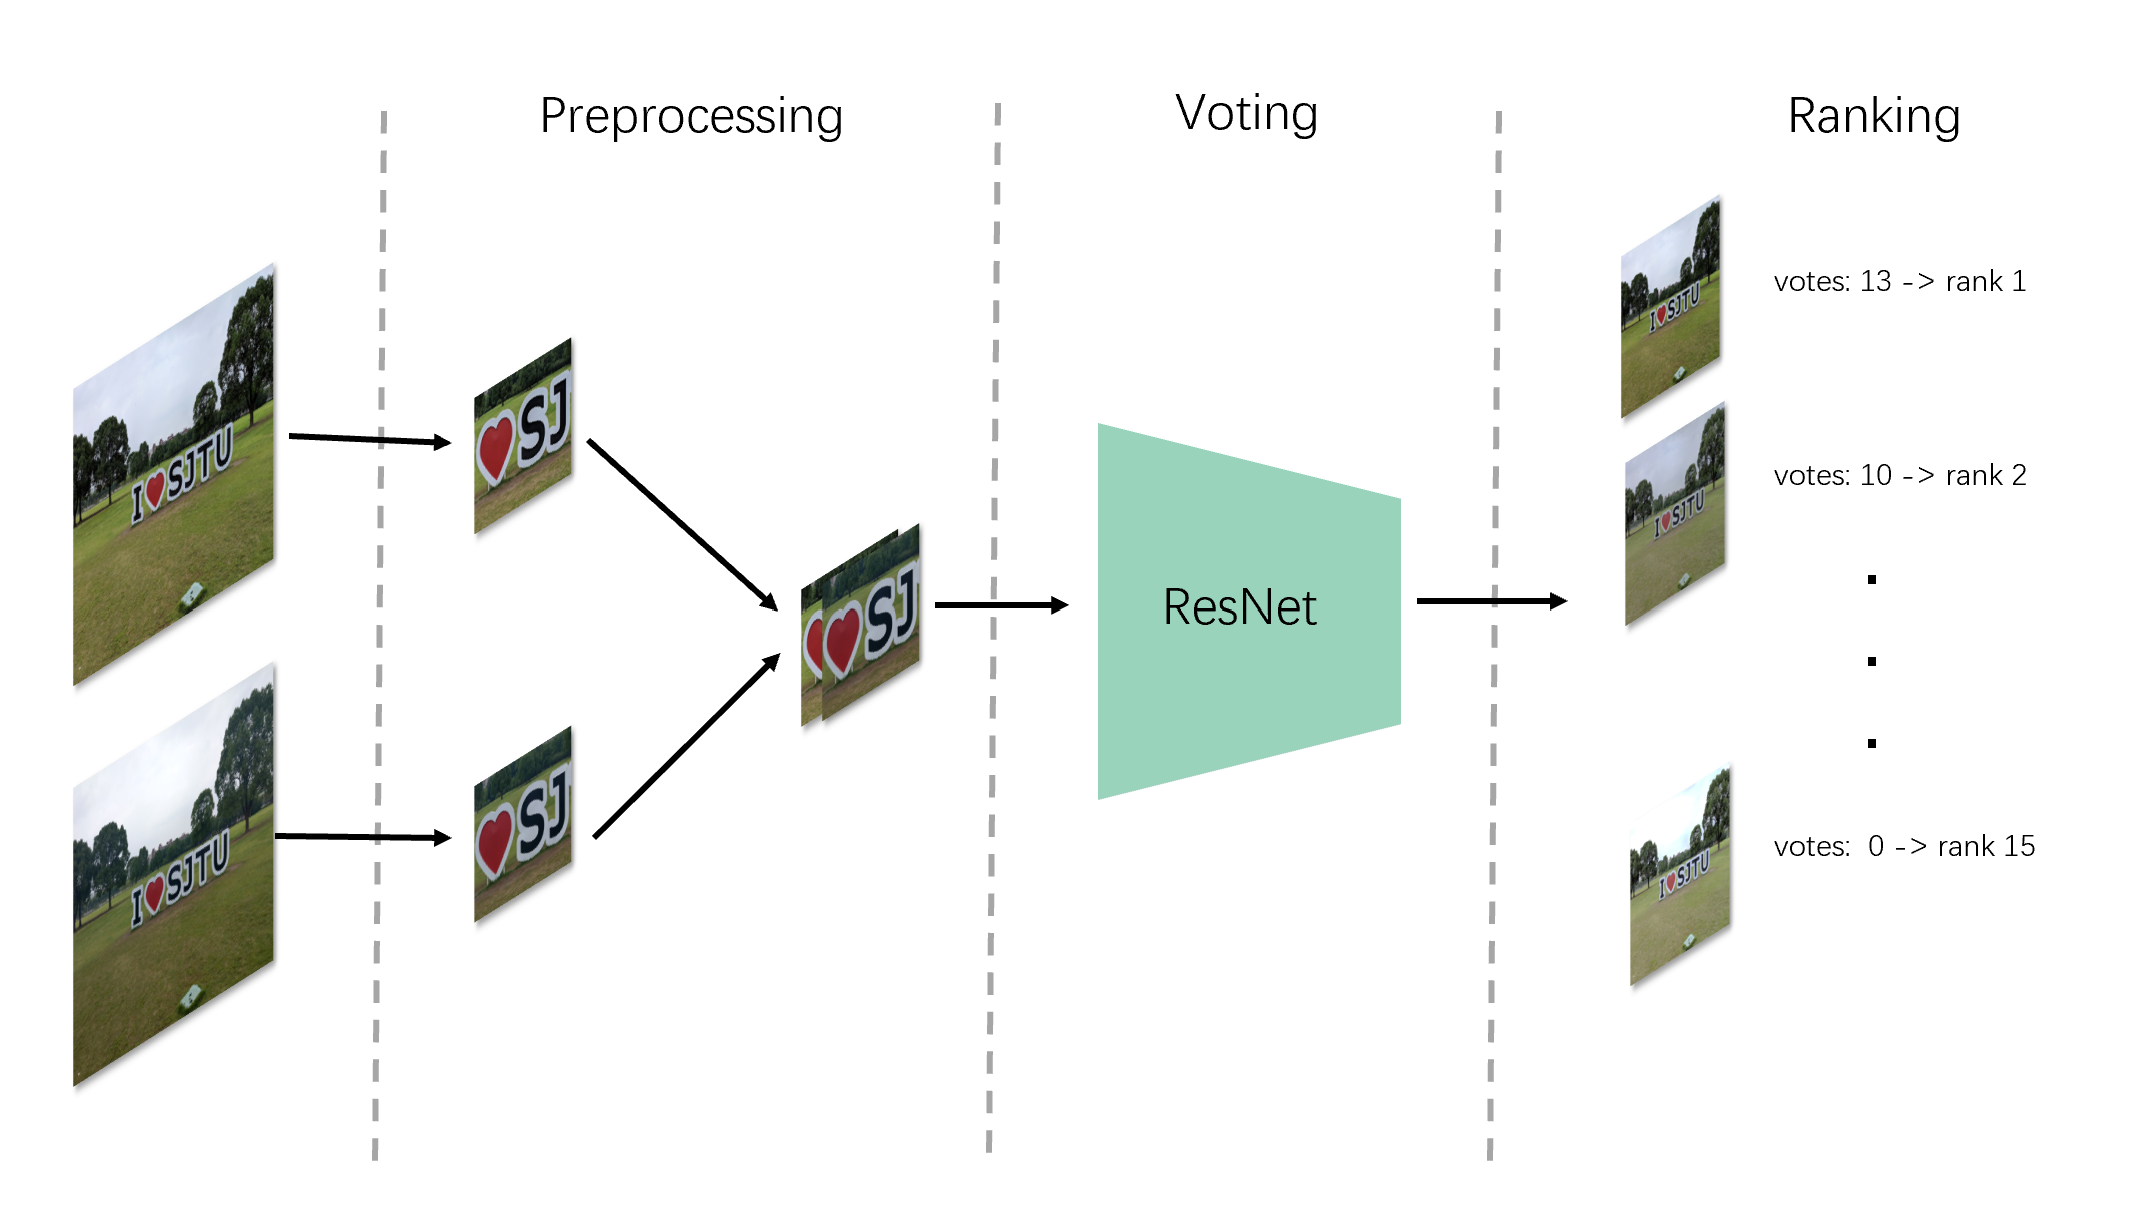
\includegraphics[width=\textwidth]{overall.png}
    \caption{The overall architecture of our proposed voting based method: for each pair of images, after preprocessing, they get stacked up as input to CNN model for voting. In the ranking stage, we rank images according to their votes.}
    \label{fig:architecture}
\end{figure*}
In this work, we formulate smartphone camera photos quality assessment as the process of image quality comparison, voting and ranking. The overall architecture of our voting based method is shown in Figure \ref{fig:architecture}.

Suppose we have a set of images taken by different devices in the same scene, $I = \{i_1, i_2, \dots, i_m\}$, where $m$ is the number of images. First, for every pair of images $(i_x, i_y) (x \neq y)$, our model compares their quality and votes for one of them:
\begin{equation}
    f(i_x, i_y) = \begin{cases}
    1, & i_x \text{ is better than } i_y\\
    0, & i_x \text{ is worse than } i_y
    \end{cases}
\end{equation}
where $f$ is a binary classification function using CNN.
After that, each image would have some number of votes (or zero vote if it's the worst image), i.e., it times of winning the comparison. Based on the voting results, we finally rank these images in an intuitive way: the more votes it has, the higher ranking it gets.

\subsection{Preprocessing}
One of the biggest challenges of smartphone camera photos quality assessment is that these photos usually have a high resolution. For example, in the SCPQD2020 database \cite{9191104}, the common resolution of smartphone camera photos is about $4000 \times 3000$, which is much higher than images used in previous NR IQA tasks.

To reduce computational costs, we need to apply some preprocessing methods rather than directly feeding entire images to CNN models. The basic idea is to crop some small patches from the original image. But how to decide which patches to crop? There are multiple possible solutions like center cropping, random cropping and other fancy techniques. But as Lu \textit{et al.}'s research \cite{9190832} shows, we gain only little benefits from carefully-designed automatic region selection. Actually, their result indicates that in most situations doing center cropping is good enough compared with automatic region selection. Therefore, in our method, we simply crop the center region from each image.

\subsection{Feature Extraction}
After preprocessing, for each pair of images, we need to extract features for further voting and ranking. It's possible to do extraction with traditional digital image processing methods, but that requires too much efforts and as Yao \textit{et al.}'s research \cite{yao2020convolutional} shows generally produces inferior results to modern deep learning methods which automatically learn more useful features. Therefore, we use convolutional neural networks to extract feature from image pairs.

As for CNNs, there are many popular choices like VGGNet \cite{simonyan2014very}, ResNet \cite{he2016deep}, ResNeXt \cite{Xie2016} and DenseNet \cite{huang2017densely}. They have all been proven powerful in image feature extraction.

In our method, we eventually choose ResNet as our CNN's backbone as it achieves a good balance between performance and computational costs. We do transfer learning \cite{pan2009survey} with pretrained ResNet models on ImageNet \cite{deng2009imagenet} to reduce training epochs. Specifically, we stack up two image patches as the input to our model, which has $2 \times 3 = 6$ channels, so we modify the first Conv2D layer of ResNet model to allow 6-channel inputs. Every following layer keeps consistent with the original ResNet model until its last fully-connected layer. We add a dropout layer \cite{srivastava2014dropout}, another fully-connected layer and finally a sigmoid layer after it. So the output of our model is a 4-dimension probability vector.

Besides, we also tried ResNet with different number of layers like ResNet18, ResNet50 and ResNet101, which will be described in more detail in Experiments section.

\subsection{Voting and Ranking Method}

For a set of images in the same scene, we feed every pair of their patches to our model. In the 4-dimension output vector, if the value in a dimension is greater than $0.5$, then we add one more vote to the first image for this dimension's corresponding metric (one of color, texture, noise and exposure). Finally, rank all these images according their votes on every metric and produce the result.

Actually, our idea for voting and ranking originally comes from Ying \textit{et al.}'s quality difference ranking model \cite{ying2020quality}. They use bubble sort to get rankings. But we think due to limits of CNN, our model might produce orders that are not topologically sort-able. For example, $i_1 > i_2, i_2 > i_3$ and $i_3 > i_1$ would make a circle. So we decide to use voting rather than sorting to address this problem.

\section{Experiments}
\subsection{Experimental Setup}
We use SCPQD2020 database \cite{9191104} to validate the performance of our proposed method. The SCPQD2020 database includes 100 scenes and in each scene there are 15 images taken by different smartphone cameras. Images in the same scene are scored and sorted in four metrics: exposure, color, noise and texture. We divide the database into three parts by scene: 70\% for model training, 10\% for model validation and 20\% for model testing. So we have $70 \times 15 \times 14 = 14700$ image pairs for training, 2100 image paires for validation and 4200 image pairs for testing. Also note that we only use images' relative rankings for training rather than their numerical scores.

In the experiments, we mainly use the Spearman Rank Order Correlation Coefficient (SRCC) as the criterion to evaluate IQA performance:
\begin{equation}
    \text{SRCC} = 1 - \frac{6\sum_{n=1}^{N}d_i^2}{N(N^2 - 1)}
\end{equation}
where $d_i$ denotes the difference between the ranks of i-th images in subjective and objective assessments, and $N$ represents the number of testing images.

SRCC is only related to the ordering of elements in the sequence. So its value indicates how much the ranking our model produces is consistent with the ground truth ranking. The larger the SRCC value, the better the performance of our model.

In the training process, we use Adam optimizer \cite{kingma2014adam} to optimize model parameters. Its learning rate is set to $1\times10^{-4}$ for both convergence and efficiency ($1\times10^{-3}$ would make our model unable to converge while $1\times10^{-5}$ is too slow). Our model is trained on a cloud server equipped with one Nvidia P4 GPU.

\subsection{Experimental Results}
In order to find out the effects of feature extraction, we experimented with CNNs of different depth. As we choose ResNet \cite{he2016deep} as our backbone CNN for feature extraction, we experimented with ResNet18, ResNet50 and ResNet101. We trained them with exactly the same experimental setup including dataset division, physical devices and hyper-parameters. Then we evaluated them on the same dataset and computed their overall SRCC on testing data. The results are shown in Table \ref{cnns}. 

We can see that ResNet50 outperforms ResNet18 obviously, but achieves similar results to ResNet101. We think the reason behind is that ResNet18 has too few layers and is not powerful enough to extract useful features for further voting and ranking while ResNet101's extra layers are of little use for our task and database. In this sense, ResNet50 is just powerful enough. But we also guess that with a larger database than SCOQD2020 \cite{9191104}, ResNet101 would possibly perform better.

Besides, it's noticeable that all these models perform relatively poorly on noise metric: they get low SRCC scores on noise. We think one possible reason is that noise is some low-level feature which ResNet is not good at extracting, compared to high-level features like color and texture. As we know, for deep CNN models like ResNet, the deeper layer, the higher-level features. Therefore, one possible solution is to use outputs from shallower layers for noise related features.

\begin{table}[]
\centering
\caption{SRCC for different backbone CNNs on the SCPQD2020 database}\label{cnns}
\begin{tabular}{llllll}
\toprule
Backbone & Color      & Exposure & Noise      & Texture  & overall  \\
\midrule
ResNet18     & 0.1102 & 0.2051 & 0.1777 & 0.1777 & 0.1677 \\
ResNet50     & 0.3048 & 0.3181 & 0.1530 & \textbf{0.2740} & 0.2624 \\
ResNet101    & \textbf{0.3142} & \textbf{0.3228} & \textbf{0.2333} & 0.2537 & \textbf{0.2810} \\
\bottomrule
\end{tabular}
\end{table}

\section{Conclusion}
In this work, we propose a voting based method with convolutional neural networks for no-reference smartphone camera photos quality assessment. We use CNN models to extract features and give votes to rank images. In addition, we experimented with several different CNNs. Our method is simple and intuitive but can achieve reasonable results.

\bibliographystyle{IEEEtran}
\bibliography{Ref}


% that's all folks
\end{document}


